\documentclass[18 pt]{beamer}
\usetheme{Madrid}
% \usefonttheme{professionalfonts}
\usefonttheme{structurebold}
\usecolortheme{rose}
\setbeamerfont{title}{size=\LARGE, series=\bfseries}
% \setbeamerfont{subtitle}{size=\large}
% \setbeamerfont{author}{size=\large}
% \setbeamerfont{date}{size=\large}
% \setbeamerfont{frametitle}{size=\Large, series=\bfseries}
% \setbeamerfont{framesubtitle}{size=\large}
% \setbeamerfont{normal text}{size=\huge}
\usepackage{enumitem}
\setlist[enumerate]{label=\arabic*)., leftmargin=*,itemsep=30pt}
\setbeamerfont{enumerate item}{size=\LARGE}
\setlist[itemize]{label=\textbullet, leftmargin=*, itemsep=5pt}

\usepackage{amsmath}
\usepackage{amssymb}
\usepackage{listings}
\usepackage{booktabs}
\usepackage{multirow}
\usepackage{multirow}
\usepackage{lmodern}
\usepackage{xcolor}
\usepackage{float}
\lstset{
  language=Python,  %代码语言使用的是matlab
  % frame=shadowbox, %把代码用带有阴影的框圈起来
  rulesepcolor=\color{red!20!green!20!blue!20},%代码块边框为淡青色
  keywordstyle=\color{blue!90}\bfseries, %代码关键字的颜色为蓝色,粗体
  commentstyle=\color{red!10!green!70}\textit,    % 设置代码注释的颜色
  basicstyle=\footnotesize,
  showstringspaces=true,%不显示代码字符串中间的空格标记
  % numbers=left, % 显示行号
  % numberstyle=8pt,    % 行号字体
  % numberstyle=\color{green},
  stringstyle=\rmfamily\slshape\color[RGB]{128,0,0}, % 代码字符串的特殊格式
  breaklines=true, %对过长的代码自动换行
  extendedchars=false,  %解决代码跨页时,章节标题,页眉等汉字不显示的问题
  escapeinside=``,%代码中出现中文必须加上,否则报错
  texcl=true}

\lstset{breaklines}%自动将长的代码行换行排版

\lstset{extendedchars=false}%解决代码跨页时,章节标题,页眉等汉字不显示的问题

\usepackage{textcomp}
% \usepackage[margin=1in]{geometry}
\usepackage{pythonhighlight}
% \usepackage{minted}
\usepackage[backend=bibtex]{biblatex}
%\usepackage[style=authortitle,backend=biber]{biblatex}
\addbibresource{ResearchRabbit_Export_2022_10_20.bib}

\usepackage{algorithm}
\usepackage{algorithmic}
\renewcommand{\algorithmicrequire}{\textbf{Input:}}
\renewcommand{\algorithmicensure}{\textbf{Output:}}

% //TODO: add
% \AtBeginSection[]{
%   \begin{frame}
%   \frametitle{Outline}
%   \tableofcontents[currentsection,hideallsubsections]
%   \end{frame}
% }
% \AtBeginSubsection[]{
%   \begin{frame}
%   \frametitle{Outline}
%   \tableofcontents[currentsubsection]
%   \end{frame}
% }
\setbeamertemplate{section in toc}{\inserttocsectionnumber.~\inserttocsection}
\setbeamertemplate{subsection in toc}[ball unnumbered]
\setbeamertemplate{subsubsection in toc}[square unnumbered]


\title{Netural Atom Quantum Computation introduction}
\author[Gcc]{Dingchao Gao}
\institute[ISCAS]{Institute of Software Chinese Academy of Sciences}

\setbeamertemplate{footline}[frame number]
\begin{document}

\begin{frame}[plain]
  \titlepage
\end{frame}
\begin{frame}{main reference}
  \begin{enumerate}
    \item Henriet, Loic, Lucas Beguin, Adrien Signoles, Thierry Lahaye, Antoine Browaeys, Georges-Olivier Reymond, and Christophe Jurczak. \textbf{Quantum Computing with Neutral Atoms}. Quantum 4 (21 September 2020): 327. \url{https://doi.org/10.22331/q-2020-09-21-327}.
    % \item Bluvstein, Dolev, Harry Levine, Giulia Semeghini, Tout T. Wang, Sepehr Ebadi, Marcin Kalinowski, Alexander Keesling, et al. \textbf{A Quantum Processor Based on Coherent Transport of Entangled Atom Arrays}. Nature 604, no. 7906 (21 April 2022): 451–56. \url{https://doi.org/10.1038/s41586-022-04592-6}.
    \item Bluvstein, Dolev, Simon J. Evered, Alexandra A. Geim, Sophie H. Li, Hengyun Zhou, Tom Manovitz, Sepehr Ebadi, et al. \textbf{Logical Quantum Processor Based on Reconfigurable Atom Arrays}. Nature 626, no. 7997 (1 February 2024): 58–65. \url{https://doi.org/10.1038/s41586-023-06927-3}.
  \end{enumerate}
\end{frame}
\section{principle}
% \begin{frame}
%   \frametitle{important principle}
%   \begin{enumerate}
%     \item Pauli exclusion principle
%     \item Aufbau principle
%     \footcite{https://en.wikipedia.org/wiki/Aufbau_principle}
%   \end{enumerate}
% \end{frame}
% some basic
% atom 
\subsection{control}
\begin{frame}{optical tweezers\footnote{\url{https://en.wikipedia.org/wiki/Optical_tweezers}}}
  \begin{columns} % The "T" option aligns the columns' content at the top

    \begin{column}{.5\textwidth} % Left column, 50% of the text width
    \begin{enumerate}[label=\arabic*., leftmargin=*, itemsep=30pt] % Customize enumerate
        \item the diameter of a trapped particle $\gg $ the wavelength of light
        \item the diameter of a trapped particle $\ll$ the wavelength of light
    \end{enumerate}
    \end{column}
    
    \begin{column}{.5\textwidth} % Right column, 50% of the text width
    \begin{figure}
      \centering
    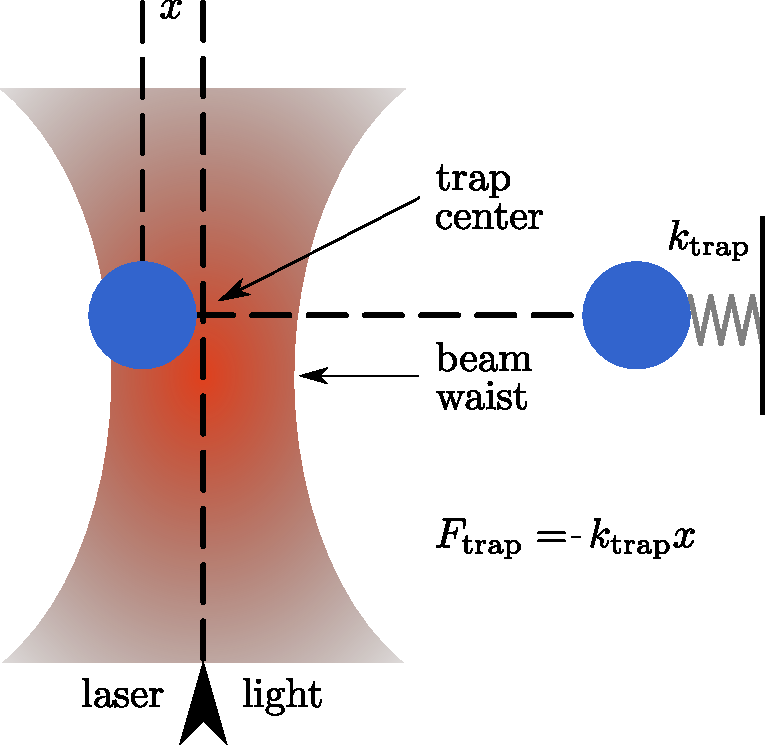
\includegraphics[width=\textwidth]{IMG/Optical_trap_prinple} % Adjust the path and image name
    \caption{Dielectric objects are attracted to the center of the beam, slightly above the beam waist}
    \end{figure}
    \end{column}
    
  \end{columns}
\end{frame}
\begin{frame}{Electric dipole approximation}
  \begin{enumerate}
    \item Induction by light (assume the dielectric particle is linear):
    \[p = \alpha \cdot E_{light}\]
    $p$ is the induced dipole moment, $E_{light}$ is the electric field of the light, and \(\alpha\) is the polarizability of the atom
    \item Gradient Force:
    \[F_{gradient} = \nabla (p \cdot E_{light})\]
  \end{enumerate}
\end{frame}
\begin{frame}{optical lattice / optical tweezers array\footnote{\url{https://en.wikipedia.org/wiki/Optical_lattice}}}
  \begin{figure}
    \includegraphics[width=.5\textwidth]{IMG/AtomsInLattice.png}
    \caption{Atoms (represented as blue spheres) pictured in a 2D-optical lattice potential (represented as the yellow surface)}
  \end{figure}
\end{frame}
\begin{frame}{AOD VS. SLM}
  \begin{enumerate}[itemsep=10pt]
    % \item Operating piciples
    % \begin{itemize}[itemsep=5pt]
    %   \item Amplitude Object Design utilize acoustic waves to diffract and control the amplitude of light waves.
    %   \item Spatial Light Modulators are devices equipped with an array of pixels, each of which can be individually controlled to alter the properties of the light. 
    % \end{itemize}
    \item \textbf{Amplitude Object Design (AOD):}
    \begin{itemize}[itemsep=5pt]
      \small
      \item \textit{Operating Principle:} Uses acoustic waves to diffract and control light's amplitude.
      \item \textit{Advantages:} Features high-speed modulation and scanning capabilities, low power consumption, and robustness for long-term use.
      \item \textit{Limitations:} Restricted to amplitude modulation without phase control, possible noise from acoustic wave generation, and efficiency dependent on material properties.
    \end{itemize}
    \item \textbf{Spatial Light Modulator (SLM):}
    \begin{itemize}[itemsep=5pt]
        \item \small \textit{Operating Principle:} Modulates light's amplitude, phase, or polarization through an array of individually adjustable pixels, enabling complex light pattern generation.
        \item \textit{Advantages:} Capable of intricate wavefront shaping and modulation across amplitude, phase, and polarization.
        \item \textit{Limitations:} Higher complexity and cost, potential diffraction artifacts due to its pixelated nature, and limited refresh rate for dynamic applications.
    \end{itemize}
  \end{enumerate}
\end{frame}

\begin{frame}{develop histroy}
  \begin{enumerate}
    \item Bose-Einstein condensate
    \item \small{Endres, Manuel, Hannes Bernien, Alexander Keesling, Harry Levine, Eric R. Anschuetz, Alexandre Krajenbrink, Crystal Senko, Vladan Vuletic, Markus Greiner, and Mikhail D. Lukin. "Atom-by-atom assembly of defect-free one-dimensional cold atom arrays." Science 354, no. 6315 (2016): 1024-1027. \url{https://www.science.org/doi/abs/10.1126/science.aah3752}.}
    \item \small{Barredo, Daniel, Sylvain de Léséleuc, Vincent Lienhard, Thierry Lahaye, and Antoine Browaeys. "An atom-by-atom assembler of defect-free arbitrary two-dimensional atomic arrays." Science 354, no. 6315 (2016): 1021-1023. \url{https://www.science.org/doi/abs/10.1126/science.aah3778}.}
  \end{enumerate}
\end{frame}
\begin{frame}{work flow}
\begin{columns}
  \begin{column}{.3\textwidth}
    \begin{enumerate}[itemsep = 10pt]
      \item metal
      \item atomic beam
      \item cooling
      \begin{enumerate}[itemsep = 5pt]
        \item zeeman slower
        \item 2D MOT
        \item 3D MOT
      \end{enumerate}
      \item optical lattice
      \item rearrange
    \end{enumerate}
  \end{column}
  \begin{column}{.7\textwidth}
    \begin{figure}
      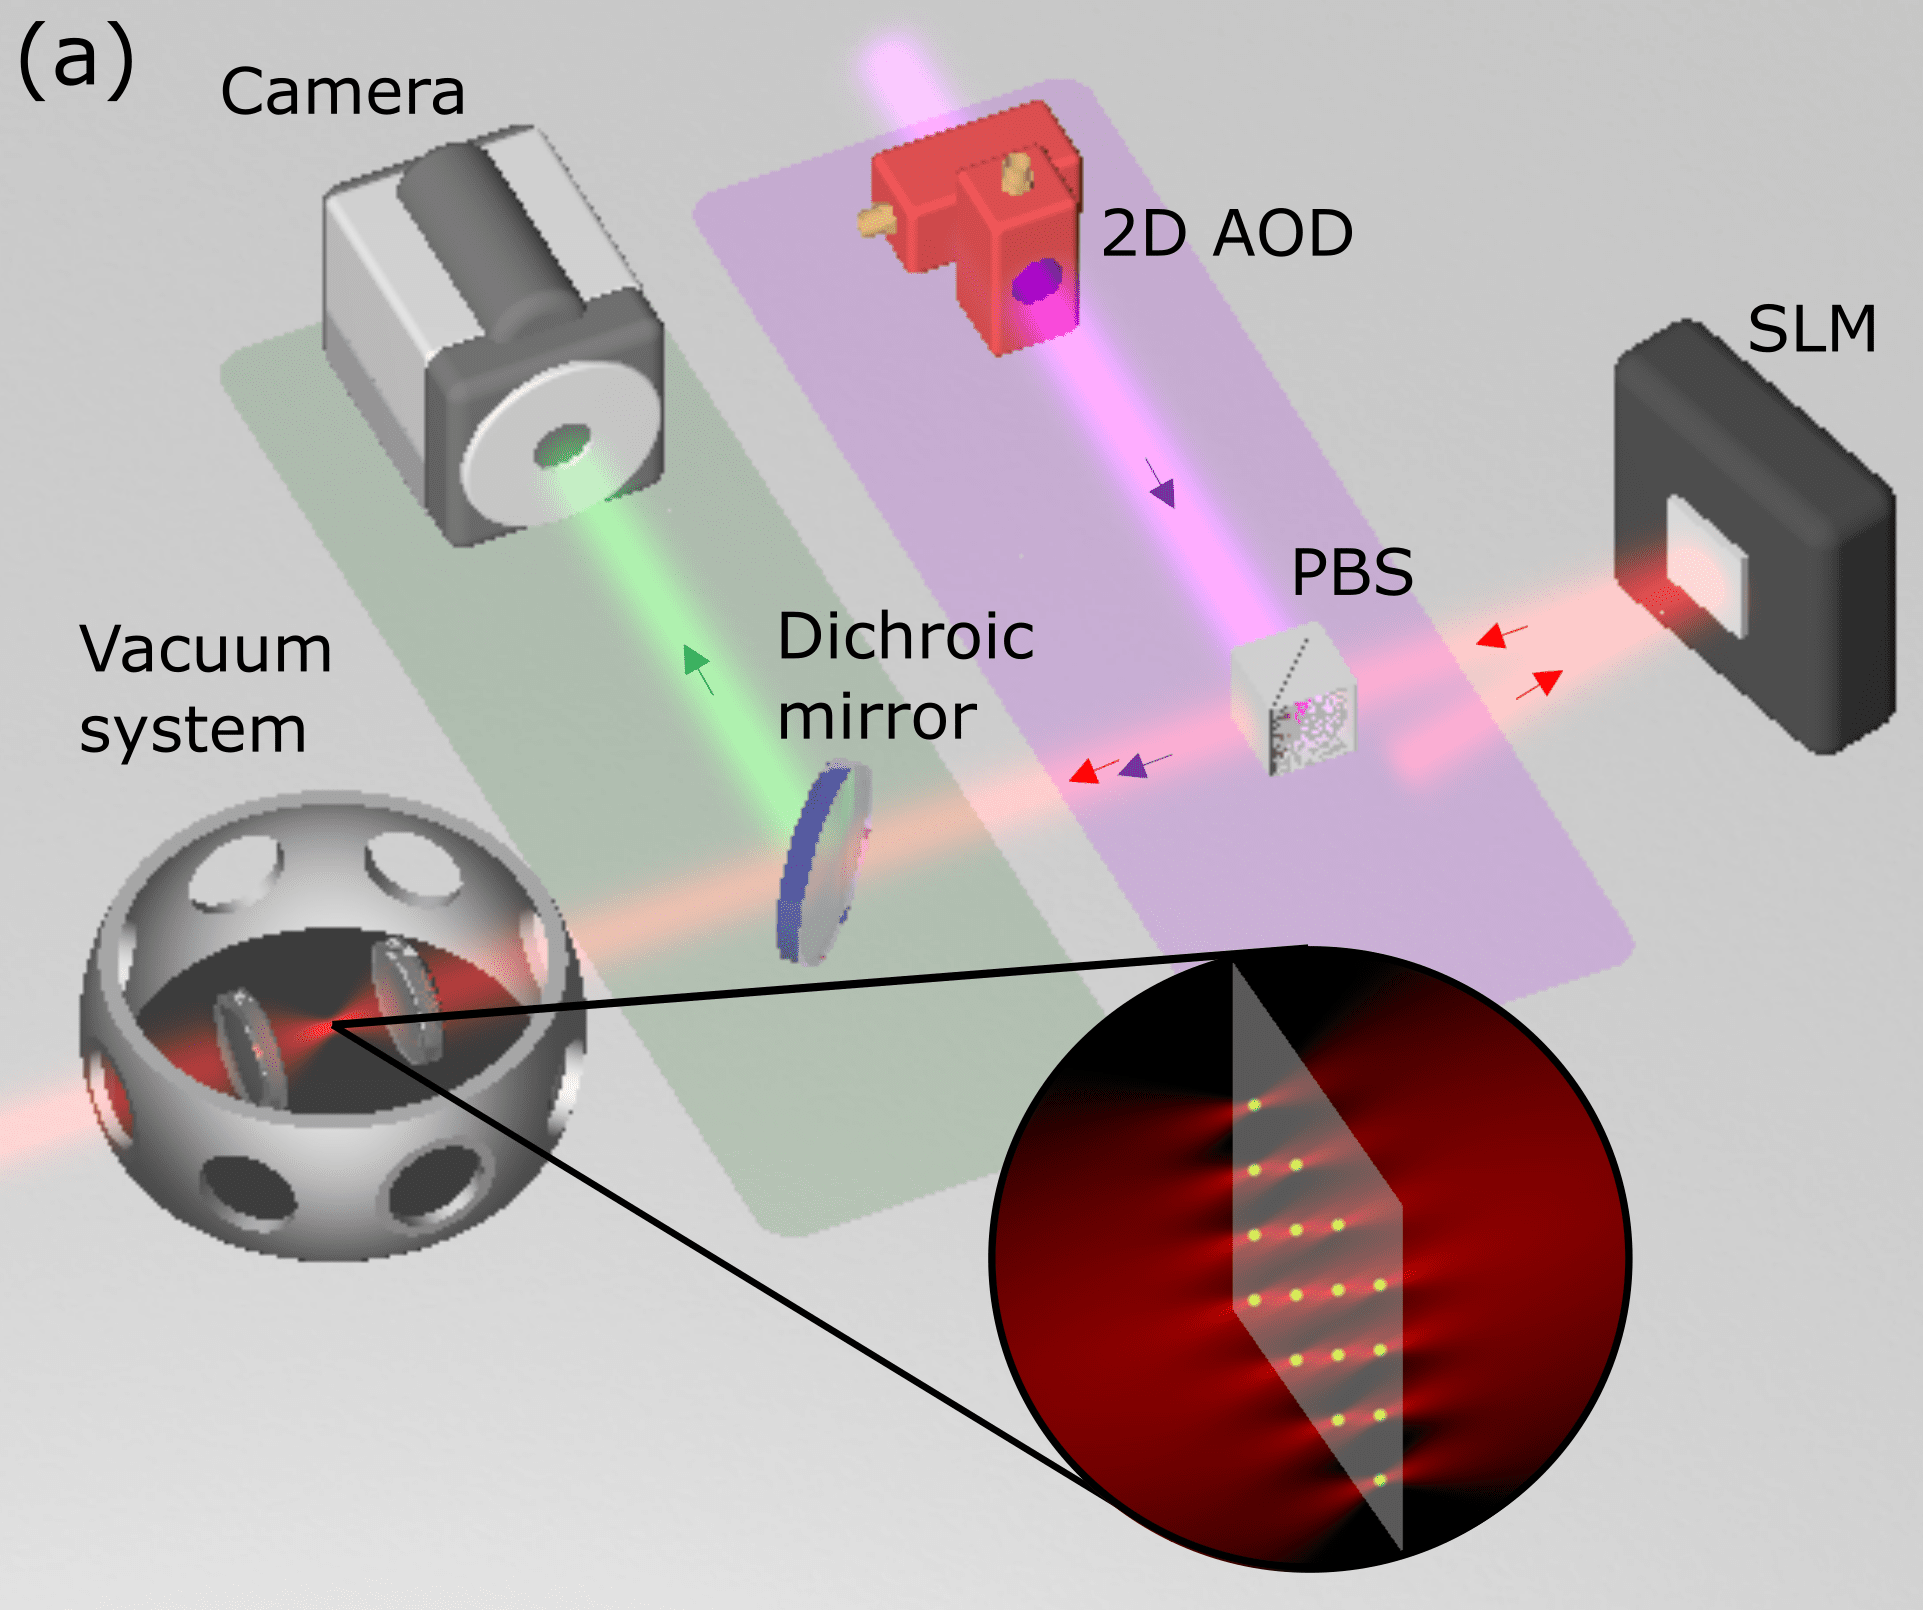
\includegraphics[width=.9\textwidth]{IMG/image.png}
      \caption{Overview of the main hardware components constituting a quantum processor}
    \end{figure}
  \end{column}
\end{columns}
\end{frame}
\begin{frame}{rearrange}
  \begin{figure}
    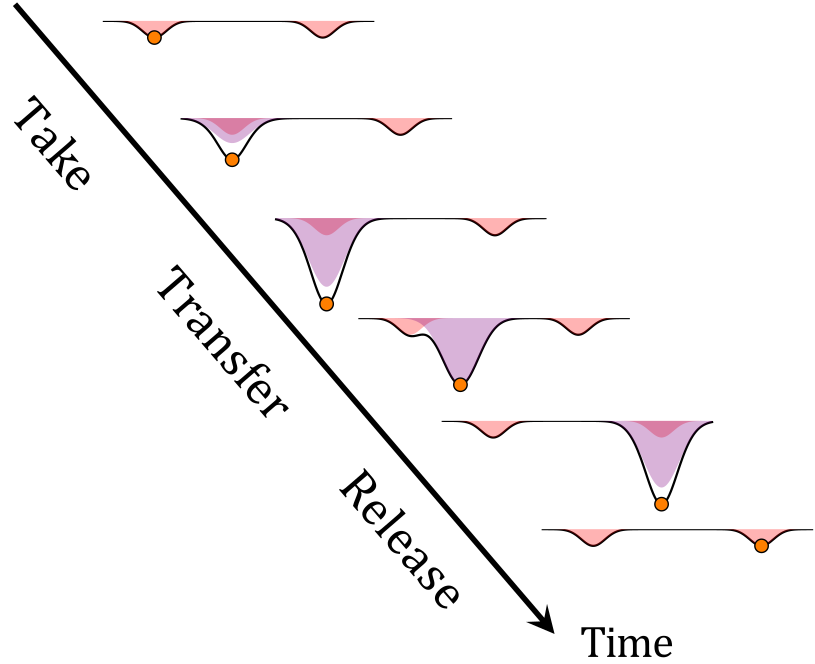
\includegraphics[width=.5\textwidth]{IMG/rearrange.png}
    \caption{Moving a single atom from one site to another (both in red) in the register}
  \end{figure}
\end{frame}
\begin{frame}{some confused words}
  \begin{enumerate}
    \item qubit sites
    \item a mean number of loading individual atoms
    \item defect-free atomic qubit clusters
  \end{enumerate}
\end{frame}

% Hamilition
\subsection{operation}
\begin{frame}{readout}
  % a example figure here
\end{frame}
\begin{frame}{single-qubit gate}
  \begin{enumerate}[itemsep=10pt]
    \item \textit{principle:} an optical laser field driving Raman transitions through an intermediate atomic state.
    \item The atom-laser interaction is characterized by:
    \begin{itemize}[itemsep = 5pt]
      \item the Rabi frequency \(\Omega\)(its strength, proportional to the amplitude of the laser field)
      \item the detuning \(\delta\) (the difference between the qubit resonance and the field frequencies) 
      \item the relative phase \(\varphi\)
      \item the duration \(\tau \)
    \end{itemize}
    \item induces rotations around the \((x,y,z)\) axes with angles \((\Omega\tau\cos{\varphi},\Omega\tau\sin{\varphi},\delta\tau)\)
  \end{enumerate}
\end{frame}
\begin{frame}{Rydberg blockade\footnote{\url{https://en.wikipedia.org/wiki/Rydberg_atom}}}
  \begin{enumerate}
    \item Van der Waals force, \(\propto R^{-6}\)
    \item dipole-dipole interaction, \(\propto R^{-3} \left( \vec{p}_1 \cdot \vec{p}_2 - 3(\vec{p}_1 \cdot \hat{R})(\vec{p}_2 \cdot \hat{R}) \right)
    \), while \(\vec{p} = q\cdot \vec{d}\)
    \item $r=\frac{n^{2}\hbar ^{2}}{ke^{2}m}$, while rydberg atoms in experiment $50\le n \le 70$
    \item two closed atoms can't be $|rr\rangle$
  \end{enumerate}
\end{frame}
\begin{frame}{how to choose atomic?}
  \begin{figure}
    \centering
    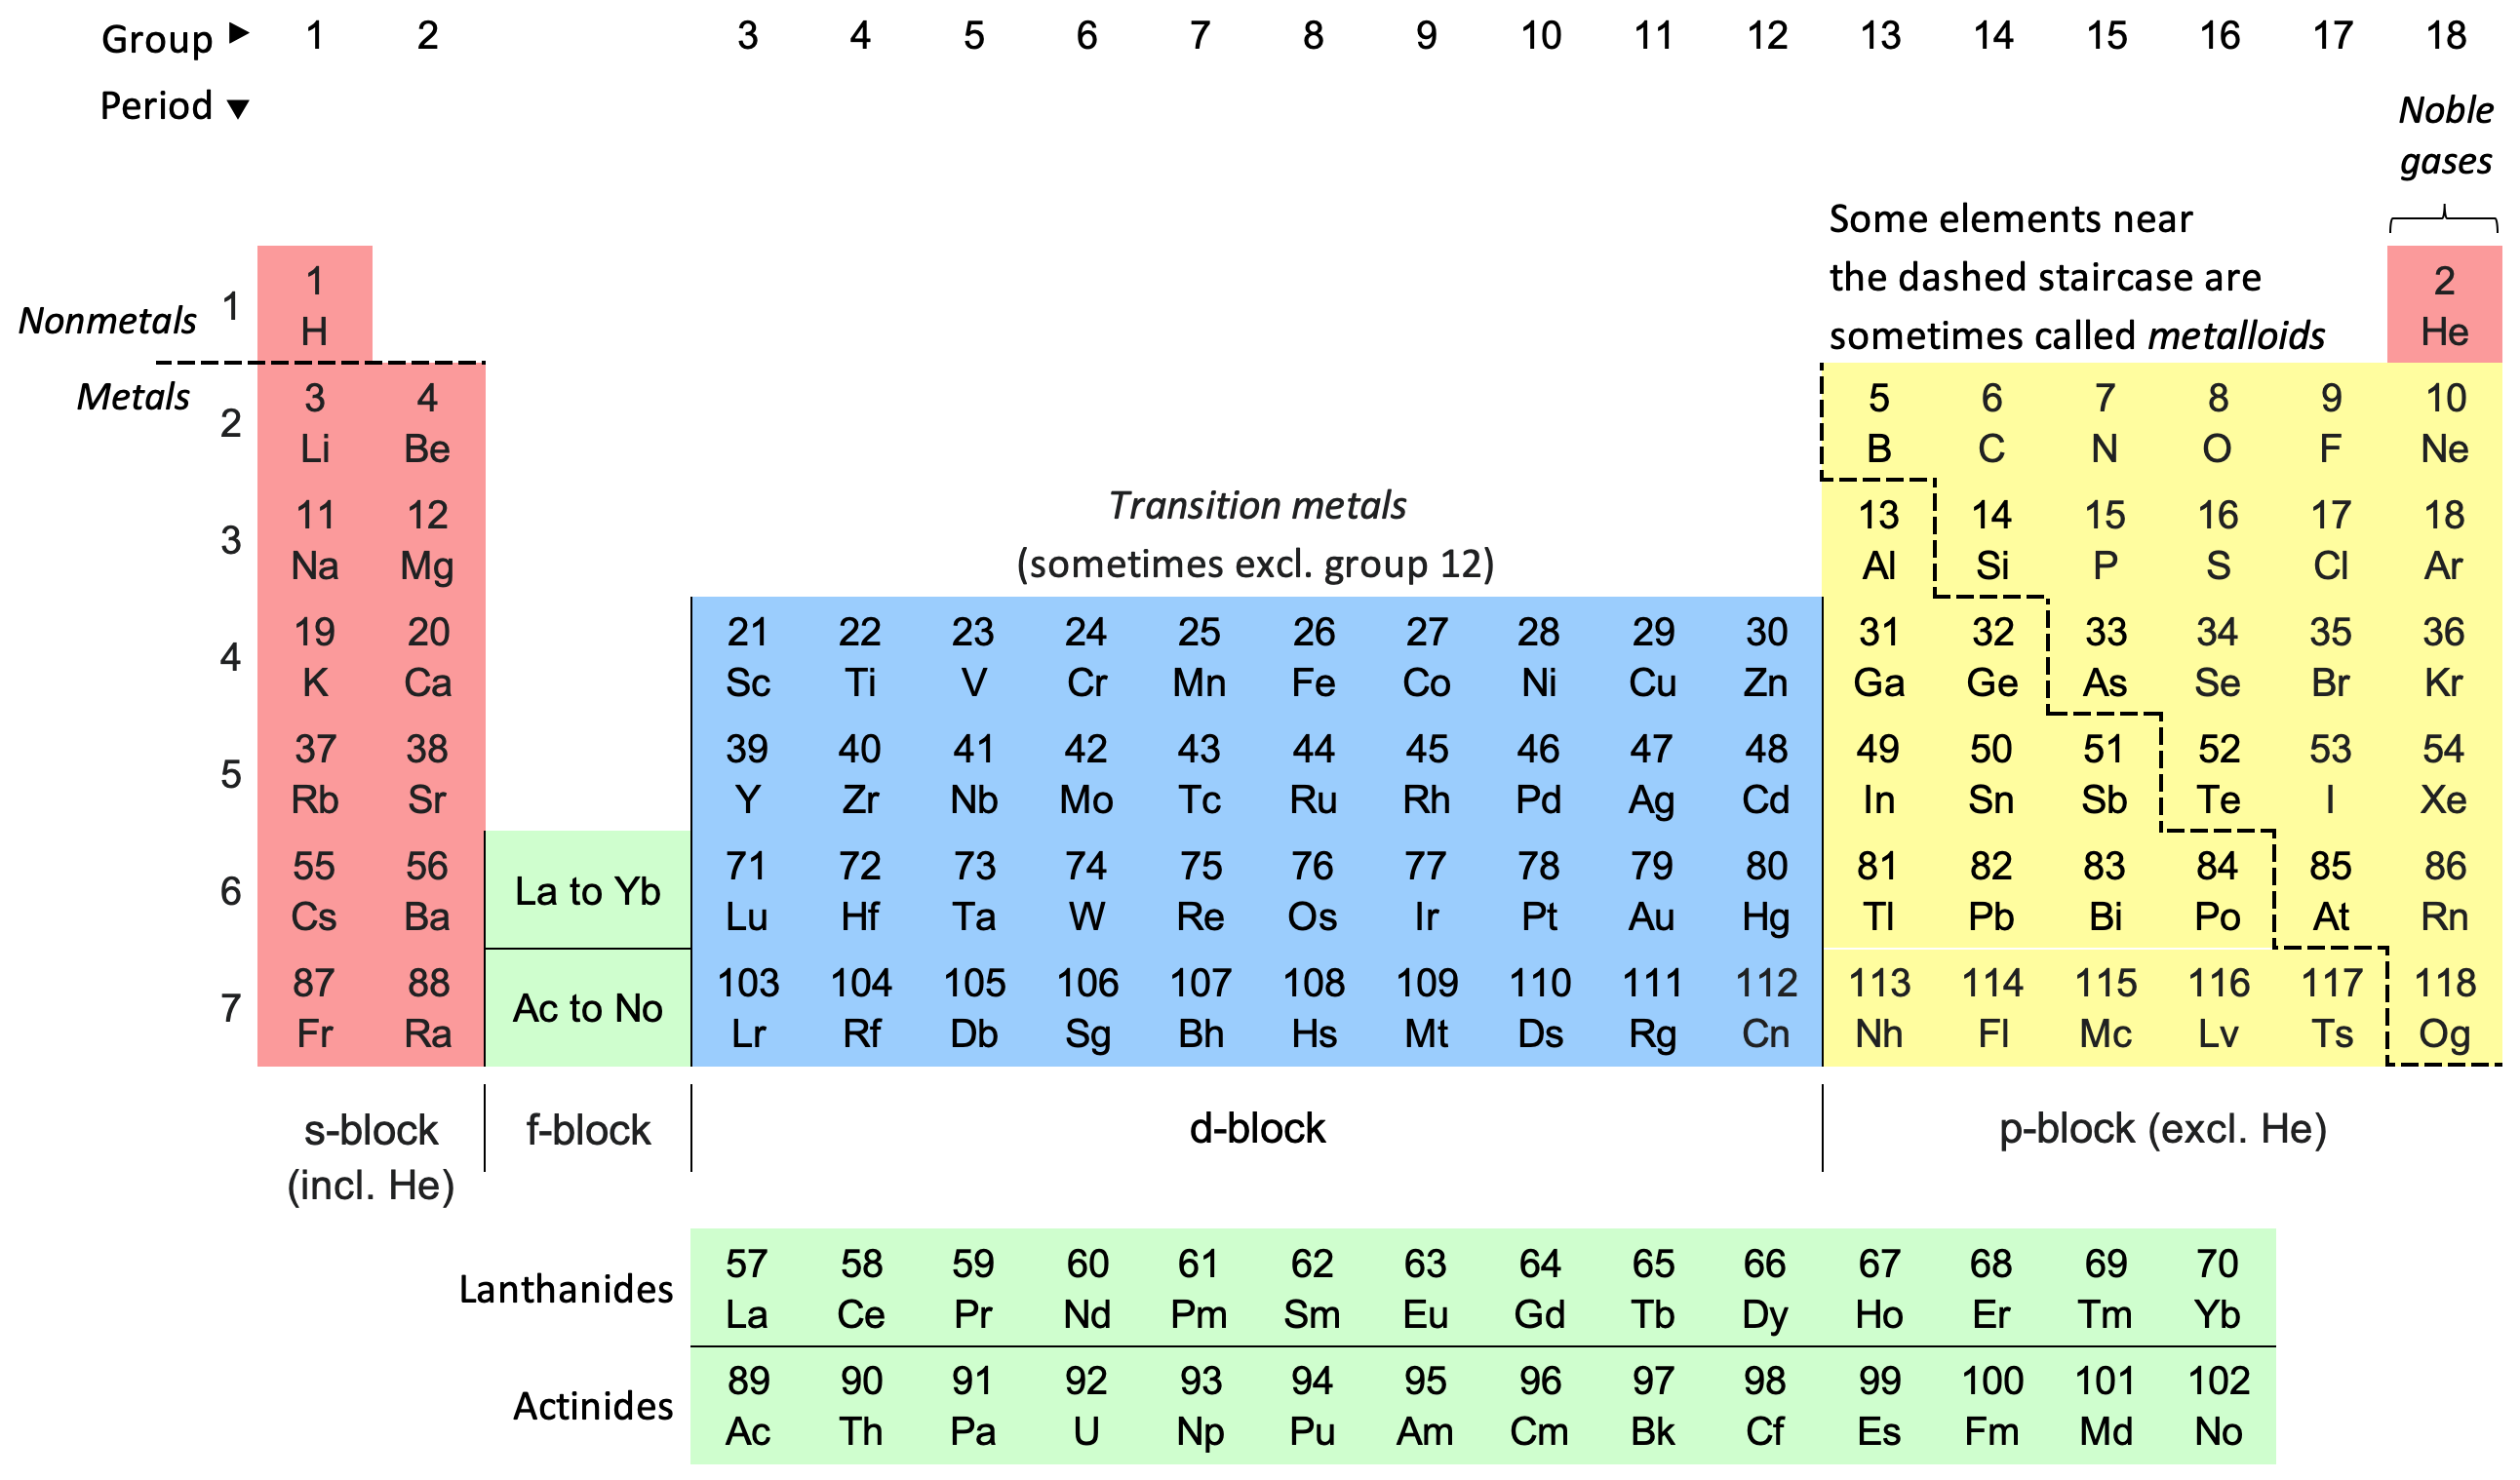
\includegraphics[width=.8\textwidth]{IMG/Colour_18-col_PT_with_labels}
    \caption{Periodic table\footnote{\url{https://en.wikipedia.org/wiki/Periodic_table}}}
  \end{figure}
\end{frame}
\begin{frame}{multi-qubit gate}
  \begin{columns}
    \begin{column}{.5\textwidth}
      realize: \(2|gg\rangle\langle gg|-\mathbb{I} \)
      \vspace{20pt}
      \begin{enumerate}
        \item \(|gg\rangle\to |gg\rangle \to |gg\rangle \to |gg\rangle\)
        \item \(|eg\rangle\to |rg\rangle \to |rg\rangle \to -|eg\rangle \)
        \item \(|ge\rangle\to |ge\rangle \to -|ge\rangle \to -|ge\rangle \)
        \item \(|ee\rangle\to |re\rangle \to |re\rangle  \to -|ee\rangle \)
      \end{enumerate}
      \vspace{20pt}
      similiar: \(2|gg\cdots\rangle\langle gg\cdots|-\mathbb{I} \)
    \end{column}
    \begin{column}{.5\textwidth}
      \begin{figure}
        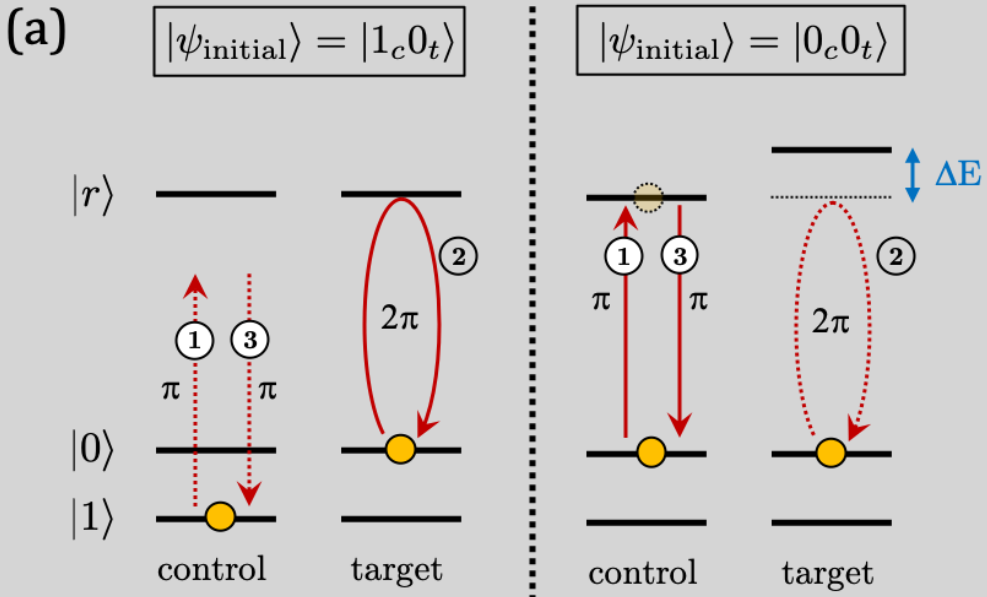
\includegraphics[width=\textwidth]{IMG/cz.png}
        \caption{Principle of the controlled-Z gate based on dipolar Rydberg interaction. First a $\pi$ pulse is applied on the control atom, then a 2$\pi$ pulse on the target atom, and finally another $\pi$ pulse on the control one.As a result, those pluses apply a gate $e^{i\pi} Z$.}
      \end{figure}
    \end{column}
  \end{columns}
\end{frame}

\begin{frame}{potential developments}
  \begin{figure}
    \centering
    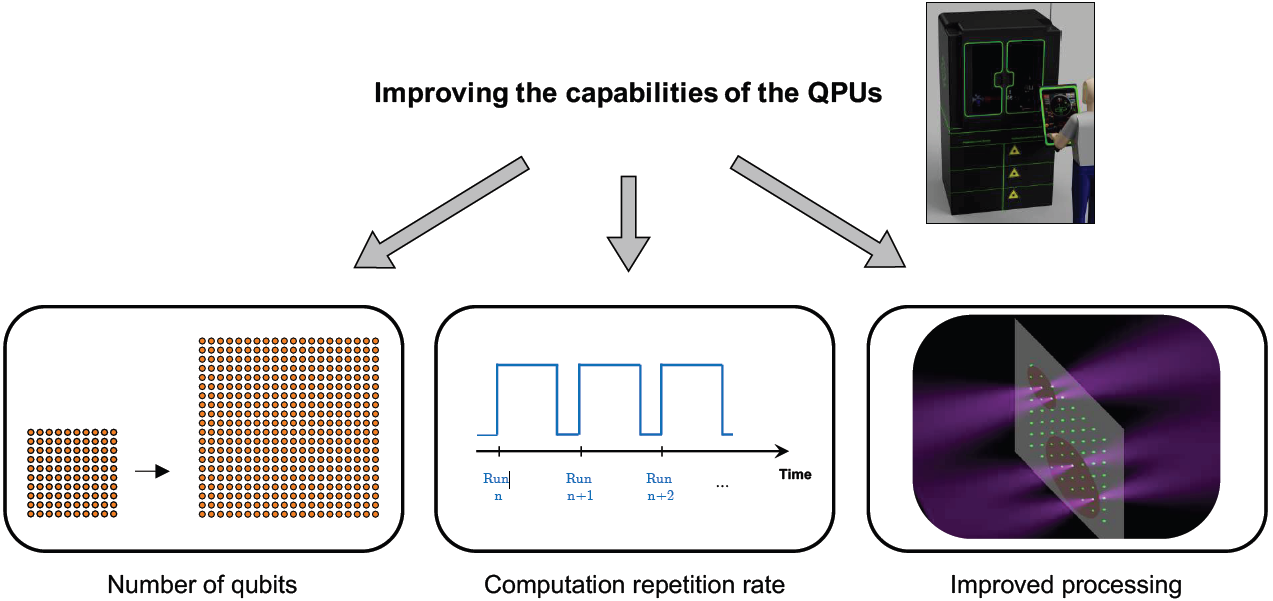
\includegraphics[width=\textwidth]{IMG/improve.png}
    \caption{The three main axes of hardware developments to improve the performances of the QPUs}
  \end{figure}
\end{frame}
% \begin{frame}{Limitations and Solutions}
%   \begin{enumerate}
%     \item \textbf{Qubit Scaling and Laser Systems}
%       \begin{itemize}[itemsep=5pt]
%         \item Higher optical power lasers for more optical tweezers.
%         \item Advanced imaging systems for larger qubit registers.
%         \item Tackling atom lifetime limitations in vacuum chambers.
%       \end{itemize}
%     \item \textbf{Overcoming Residual Pressure Limitations}
%       \begin{itemize}[itemsep=5pt]
%         \item Compact cryogenic QPUs for extended atom lifetimes.
%         \item Faster operation cycles to outpace decoherence.
%       \end{itemize}
%   \end{enumerate}
% \end{frame}

\begin{frame}{technological enhancements}
  \begin{enumerate}[itemsep=15pt]
    \item Higher optical power lasers for more optical tweezers.
    \item Advanced imaging systems for larger qubit registers.
    \item Overcoming Residual Pressure Limitations
    \item Enhanced atomic sources for quicker register loading.
    \item High-bandwidth electronics for precise operation control.
  \end{enumerate}
\end{frame}
\section{device}
\subsection{scalability}
\begin{frame}{breakthrough}
  \begin{enumerate}[itemsep=10pt]
    \item Pause, Lars, Lukas Sturm, Marcel Mittenbühler, Stephan Amann, Tilman Preuschoff, Dominik Schäffner, Malte Schlosser, and Gerhard Birkl. \textbf{Supercharged Two-Dimensional Tweezer Array with More than 1000 Atomic Qubits}. Optica 11, no. 2 (7 February 2024): 222. \url{https://doi.org/10.1364/OPTICA.513551}.
    \item Norcia, M. A., H. Kim, W. B. Cairncross, M. Stone, A. Ryou, M. Jaffe, M. O. Brown, et al. \textbf{Iterative Assembly of $^{171}$Yb Atom Arrays in Cavity-Enhanced Optical Lattices}. arXiv, 9 February 2024. \url{http://arxiv.org/abs/2401.16177}.
    \item Gyger, Flavien, Maximilian Ammenwerth, Renhao Tao, Hendrik Timme, Stepan Snigirev, Immanuel Bloch, and Johannes Zeiher. \textbf{Continuous Operation of Large-Scale Atom Arrays in Optical Lattices}. arXiv, 10 February 2024. \url{http://arxiv.org/abs/2402.04994}.
  \end{enumerate}
\end{frame}
\begin{frame}{supercharged}
\begin{figure}
  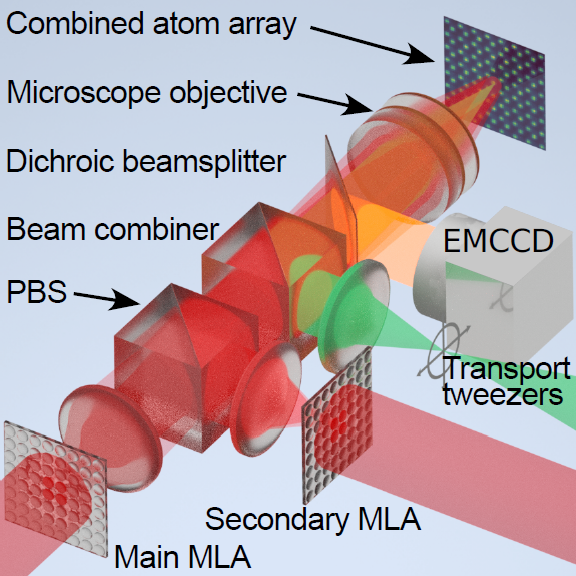
\includegraphics[width=.5\textwidth]{IMG/supercharhed.png}
  \caption{In the experimental setup described in the paper titled \textit{Supercharged}, the implementation encompasses 3000 qubit sites, including 441 qubits, utilizing Rubidium (Rb) as the core element.}
\end{figure}  
\end{frame}
\begin{frame}{Atom Computing}

\end{frame}
\begin{frame}{Max-Planck-Institut}
\end{frame}
\begin{frame}{summarize}
\end{frame}
\subsection{error correction}
\begin{frame}{set up}
\end{frame}
\section{synthess}
\begin{frame}{discussion}
\end{frame}
\end{document}